
\documentclass[ngerman, twoside]{tudscrreprt}

\usepackage{mystyle}

% \includeonly{tex/preembel, ...}

\begin{document}

\subject{bachelor}
\faculty{Fakultät Informatik}
\institute{Institut für Systemarchitektur}
\chair{Lehrstuhl für Datenbanken}
\date{18.07.2017}
\author{Lucas Kuhring}
\matriculationnumber{4038042}
\title{Untersuchung von Intel SGX für eine sichere Verarbeitung komprimierter Daten}
\supervisor{Dr.-Ing. Dirk Habich}
\professor{Prof. Dr.-Ing. Wolfgang Lehner}
\maketitle
\TUDoption{abstract}{single,fill,notoc}

\cleardoublepage

% Selbstständigkeitserklärung
\confirmation

\cleardoublepage

\pagenumbering{roman}

% 0. Abstract

\begin{abstract}
	\section*{Abstract}
	The storage and processing of data in a cloudbased environment is a challenging task from a security perspective. Remote systems cannot be fully trusted and might involve privileged software components corrupted by an adversary, willing to collect the stored data. Intel Software Guard Extensions (SGX) are the processing hardware vendor's approach to allow the work on data in a protected region in memory, leaving the Intel processor as the only part of the system, that has to be trusted. From a development point of view a officially released SDK offers an intuitive way to use the protected memory by defining 'Enclaves' as independent units that live inside of it. Functions that process sensitive data are declared as part of an enclave, that is later included as a library by an ordinary application, making calls to its interface.
	%TODO of course that has to be done at the end :)
\end{abstract}

\tableofcontents
\newpage

\listoffigures
\listoftables

% Abkürzungsverzeichnis

\chapter*{Abkürzungsverzeichnis}

\begin{acronym}[DBMS]
	\acro{AES}{Advanced Encryption Standard}
	\acro{AVX}{Advanced Vector Extensions}
	\acro{BIOS}{Basic Input/Output System}
	\acro{CBC}{Cipher Block Chaining}
	\acro{CPU}{Central Processing Unit}
	\acro{DBMS}{Database Management System}
	\acro{DLL}{Dynamic Link Library}
	\acrodefplural{DLL}{Dynamic Link Libraries}
	\acro{ECall}{Enclave Call}
	\acro{EDL}{Enclave Definition Language}
	\acro{EPC}{Enclave Page Cache}
	\acro{EPCM}{Enclave Page Cache Map}
	\acro{FPGA}{Field Programmable Gate Array}
	\acro{MIPS}{Million Instructions per Second}
	\acro{OCall}{Out Call}
	\acro{PRM}{Processor Reserved Memory}
	\acro{RLE}{Run Length Encoding}
	\acro{SDK}{Source Development Kit}
	\acro{SECS}{SGX Enclave Control Structure}
	\acro{SGX}{Software Guard Extensions}
	\acro{SIMD}{Single Instruction, Multiple Data}
	\acro{SO}{Shared Object}
	\acro{SQL}{Structured Query Language}
	\acro{TCB}{Trusted Computing Base}
	\acro{TCS}{Thread Control Structure}
	\acro{TLS} Transport Layer Security
	\acro{tRTS}{Trusted Runtime System}
	\acro{UDF}{User Defined Function}
	\acro{uRTS}{Untrusted Runtime System}
	\acro{XML}{Extensible Markup Language}
\end{acronym}

\pagenumbering{arabic}
% 1. Einleitung

\chapter{Einleitung}

Die Erhebung und Speicherung von Daten ist eine seit den letzten Jahren ständig wachsende Entwicklung. "`Big Data"' ist eines der zentralen Schlagworte des Bereichs Data Science und umschreibt jenen Prozess. Um den großen Mengen an Daten Herr zu werden, sind immer umfangreichere Speicher- und Rechenkapazitäten nötig. Viele Unternehmen setzen daher schon seit einigen Jahren auf die Nutzung von Diensten in der Cloud, um jene erforderliche Infrastruktur auszulagern. Die Wartung von Servern wird dabei einem unabhängigen Drittanbieter überlassen. Dieses als Database-as-a-Service betitelte Modell bringt für die Firmen neben den Vorteilen der Entlastung aber auch große Risiken mit sich, denn in vielen Fällen handelt es sich um die Speicherung und Verarbeitung von sensitiven Daten, welche sich fortan auf nicht vertraulichen Systemen befinden. Ein offensichtliches Vorgehen ist die komplette Verschlüsselung der Datenbanken. Dies stellt sich aber als äußerst unpraktikabel heraus, da jene Daten auch verarbeitet werden müssen, also lesend und schreibend auf sie zugegriffen werden muss. Dies sollte jedoch aufgrund der potenziellen Komplexität nicht erst auf dem anfragenden Client geschehen.

In der Vergangenheit haben sich zwei generelle Ansätze zur Lösung dieses Problems herausgestellt. Zum einen setzt man auf spezielle Verschlüsselungsverfahren, welche Berechnungen auf Schlüsseltexten erlauben, jedoch auf Kosten der kryptographischen Sicherheit, des Berechnungsaufwands oder der Funktionalität. Auf der anderen Seite versucht man, Daten in gewisse Vertrauensbereiche zu transferieren, um sie dort sicher verarbeiten zu können. Oftmals handelt es sich hierbei um sichere Hardwarekomponenten. Innerhalb jener Bereiche entschlüsselt man die Daten, führt entsprechende Berechnungen auf ihnen aus und verschlüsselt sie wieder, bevor sie den Bereich verlassen. Die Nachteile hierbei liegen im oftmals stark eingeschränkten Speicherplatz, der für Berechnungen zur Verfügung steht. Eine Kombination der zwei Herangehensweisen vermindert die Nachteile auf beiden Seiten, und wird von den meisten aktuellen Ansätzen genutzt.
 
Intel stellt mit den \ac{SGX} eine Menge von Erweiterungen für ihre Prozessorarchitektur bereit, welche das Ziel verfolgen, die sichere Datenverarbeitung zu ermöglichen. Sie erlauben es dem Entwickler sogenannte Enclaves zu definieren. Dies sind Vertrauensbereiche, in welchen eine sichere Berechnung auf Daten ermöglicht wird, während sämtliche privilegierte Software im System, etwa der Betriebssystemkern, gleichzeitig korrumpiert sein kann. Lediglich der Prozessor hat die Möglichkeit, Einsicht in die Daten innerhalb von Enclaves zu erhalten. Somit lässt sich Intel \ac{SGX} klar in die Kategorie der auf Vertrauensbereichen basierenden Ansätze einordnen.

Während sich herkömmliche Einsatzfälle eher darauf beschränken, einzelne sensible Daten wie Passwörter in einer Enclave zu halten, soll Intels Technologie in dieser Arbeit im Kontext einer In-Memory Datenbank untersucht werden. Es handelt sich hierbei um Systeme, welche hauptsächlich innerhalb des Hauptspeichers arbeiten und somit eine deutlich schnellere Datenverarbeitung erlauben. Aufgrund von stets billiger gewordenem Arbeitsspeicher haben sie sich als Alternative zu herkömmlichen, auf Festplattenspeicher arbeitenden Systemen bewährt. Das Ziel ist es, auf Grundlage konkreter Fragestellungen zu untersuchen, ob es möglich ist die komplette Anfrageverarbeitung einer solchen Datenbank in eine sichere Enclave zu verlagern und dies mit Augenmerk auf den zusätzlichen Bearbeitungsaufwand auf seine Sinnhaftigkeit zu prüfen. Interessant ist etwa, ob der zeitliche Overhead im Gegensatz zu einer konventionellen, aber unsicheren Verarbeitung vernachlässigbar ist. Um die Berechnungsgeschwindigkeit innerhalb einer Enclave zu maximieren, ist es unter Umständen nötig, sehr große Datenmengen gleichzeitig zu halten. Wie bereits in In-Memory Datenbanken gängig, soll ein auf diese Weise potenziell auftretendes Platzproblem durch den Einsatz von leichtgewichtigen Kompressionsverfahren gelöst werden. Der Aufwand von Datenkompression könnte um einiges geringer sein, als ein ständiges Transferieren neuer Daten in die Enclave. Zudem existieren Verfahren wie die Lauflängenkodierung, welche ein teilweise schnelleres Rechnen auf komprimierten Daten erlauben. Jene Kompressionsverfahren kommen während der Untersuchungen zum Einsatz.

Für die Bearbeitung dieses Themas ist die Arbeit grundsätzlich zweigeteilt. Der erste Teil umfasst Kapitel 2 und 3, welche zunächst eine theoretische Grundlage legen sollen. In Kapitel 2 wird zum ersten auf das Thema der Sicherheit in Datenbanken eingegangen. Im Vordergrund steht die Betrachtung zentraler Begriffe aus der Datensicherheit und ein konzeptioneller Überblick über Intel \ac{SGX}. Zudem werden verwandte Arbeiten behandelt, die sich ebenso eine sichere Datenverarbeitung zum Ziel gesetzt haben. Das folgende Kapitel handelt vom Begriff der Datenkompression, und setzt diesen in den Kontext der Arbeit. Auch hier werden grundlegende Konzepte erklärt und auf verwandte Arbeiten eingegangen. Mit VByte und der Lauflängenkodierung werden zudem konkrete Kompressionsalgorithmen behandelt, welche für spätere Untersuchungen relevant sind. Der zweite große Teil umfasst Kapitel 4-6 und ist primär praktisch orientiert. Im Fokus stehen hier die eigenen Untersuchungen, angefangen mit Kapitel 4 und einer Beschreibung der Implementierung einer Anwendung unter Nutzung von \ac{SGX}. Die Betrachtung verschiedener Tests und Auswertung der entstandenen Ergebnisse erfolgt nachfolgend in Kapitel 5. Abschließend werden in einem Fazit die erlangten Erkenntnisse zusammengefasst und ein Ausblick auf weiterführende Themen und Fragestellungen gegeben.
% 2. Sicherheit in Datenbanken

\chapter{Sicherheit in Datenbanken}

Um grundsätzlich ein System in Bezug auf seine (Informations-)sicherheit zu betrachten, ist es notwendig, dieses auf die Einhaltung gewisser Merkmale hin zu charakterisieren. Diese als Schutzziele bezeichneten Eigenschaften fallen je nach Kontext anders aus. Im Allgemeinen bestehen sie jedoch den drei Begriffen Vertraulichkeit, Integrität und Verfügbarkeit:

\paragraph{Vertraulichkeit}
Als Vertraulichkeit bezeichnet man die Eigenschaft, dass Informationen in einem System nur denjenigen Subjekten zur Verfügung steht, welche dazu berechtigt sind.

\paragraph{Integrität}
Integrität liegt vor, wenn jegliche Modifikation einer Datenmenge zu jeder Zeit erkannt werden kann.

\paragraph{Verfügbarkeit}
Ein System besitzt Verfügbarkeit, wenn es fortlaufend unter korrekter Funktionsweise verfügbar ist.

\paragraph{}
Dieses Kapitel beschäftigt sich zunächst mit dem konventionellen Vorgehen zur Gewährleistung der Schutzziele in Datenbanksystemen. Um die Problematik dieser Arbeit aufzugreifen, wird daraufhin auf die Sicherheitsaspekte von Datenbanklösungen in nicht vertrauenswürdigen Umgebungen eingegangen, wobei relevante Begriffe erklärt werden. Nachfolgend erfolgt eine Darstellung entsprechender Lösungskonzepte aus anderen Publikationen. Zum Abschluss des Kapitels wird der Fokus auf das Konzept und den grundlegenden Aufbau von Intel SGX, den in dieser Arbeit untersuchten Ansatz, gelegt.

\section{Konventionelles Lösungskonzept}

Um Sicherheit in einem Datenbanksystem zu erreichen setzte man klassischerweise auf ein schichtweise organisiertes Konzept, dessen Basis durch den physischen Schutz der Systemhardware gebildet wird. Die nächsthöhere Ebene bildet das Betriebssystem, welches wiederum eigene Maßnahmen zur Verfügung stellt um das Datenbanksystem zu schützen. Letzteres bildet die oberste Ebene und gleichzeitig die Schnittstelle zum Benutzer. Jede Ebene ist auf die Gewährleistung von Sicherheit aus der jeweils unterliegenden Schicht angewiesen. Gelingt einem Angreifer etwa der physische Zugriff auf das System, so sind weder die Maßnahmen des Betriebssystems, noch des Datenbanksystems wirkungsvoll. Entsprechender Schutz wird durch klassische Mittel wie dem Einsatz von Sicherheitspersonal, Alarmsystemen und sonstiger physischer Zugriffskontrolle der Hardware gewährleistet. Auf der Ebene des Betriebssystem werden Authentisierungsverfahren genutzt, um den Zugriff abzusichern. Üblicherweise handelt es sich hierbei um Anmeldedaten, welche aus einer Nutzeridentifikation um einem Passwort bestehen. Außerdem stehen \textit{Auditing Services} zur Verfügung, welche es erlauben, Änderungen des Systemzustandes anhand von Logs nachzuvollziehen, was der Einhaltung von Integrität zugute kommt. Zuletzt ist auch das Datenbanksystem selbst dafür zuständig, die eigene Sicherheit zu schützen. Die Funktionalitäten des Betriebssystems sind hierfür allein nicht ausreichend, was vor allem dadurch begründet ist, dass oftmals komplexe Beziehungen zwischen den gespeicherten Daten zusätzliche Semantik hinzufügen, welche in der unterliegenden Ebene nicht existiert. Die Organisation der Datenobjekte erfolgt entsprechend auf einer höheren Abstraktionsebene, als dies innerhalb des Betriebssystems in Form von Dateien der Fall ist \cite{Vimercati2001}. Zur Gewährleistung von Vertraulichkeit und Integrität sind demnach auch hier eine gesonderte Zugriffskontrolle und Auditing notwendig.

Die einfache Zugriffsregelung zum Schutz der Vertraulichkeit stellt eine große Schwäche des betrachteten Konzeptes dar, da ein privilegierter Nutzer, etwa ein böswilliger Datenbank- oder Systemadministrator, die Einsicht über jegliche Daten besitzt. Vor allem aber der verstärkt genutzte Einsatz von Datenbanklösungen in einer nicht vertraulichen Cloudumgebung machen jenen Ansatz obsolet, da sich das genutzte \ac{DBMS} auf dem System des jeweiligen Anbieters befindet. Die untergeordneten Schichten sind demzufolge außerhalb der eigenen Kontrolle, woraus sich die Notwendigkeit ergibt, dass sich allein das Datenbanksystem um die Einhaltung von Vertraulichkeit und Integrität kümmern muss. In Abbildung \ref{fig:dbsecurity} ist die Relation zwischen den drei Schichten \ac{DBMS}, Betriebssystem und physischer Hardware dargestellt, wobei das klassische mit einem cloudbasierten Szenario (Database-as-Service) verglichen wird. Umrahmte Bereiche stellen den jeweiligen Einflussbereich dar.

\begin{figure}
	\includegraphics[width=0.8\linewidth]{img/DBSecurity.pdf}
	\centering
	\caption{Einflussbereich in der Systemhierarchie}
	\label{fig:dbsecurity}
\end{figure}

\section{Datenbanksicherheit in nicht vertrauenswürdigen Umgebungen}

Im Kontext dieser Arbeit wird konkret ein Datenbanksystem betrachtet, welches sich zwar unter der Kontrolle einer berechtigten Partei, jedoch in einem nicht vertrauenswürdigen Umfeld befindet. Da es hierbei hauptsächlich um die Vertraulichkeit in Bezug auf sensitive Daten geht, werden Integrität und Verfügbarkeit im Folgenden stets außer Acht gelassen. Die Speicherung jener Daten auf einem Datenbankserver offenbart allgemein drei kritische Szenarien, welche zum Schutz der Vertraulichkeit gezielt betrachtet werden müssen \cite{Shmueli2010}. Hierbei wird zunächst angenommen, es handelt sich um ein klassisches Datenbanksystem, welches Daten vordergründig auf der Festplatte speichert.

\paragraph{Data-in-motion}
Die Kommunikation zwischen Client und Server, wobei standardmäßige Kommunikationsprotokolle zum Einsatz kommen.

\paragraph{Data-in-use}
Daten, welche zum aktuellen Zeitpunkt verarbeitet werden, liegen im Hauptspeicher und können dort durch einen Angreifer ausgelesen werden.

\paragraph{Data-at-rest}
Gespeicherte Daten befinden sich auf der Festplatte und müssen vor unbefugtem Zugriff geschützt werden.

\paragraph{}
Aufgrund standardisierter Protokolle zur sicheren Client-Server Kommunikation (\ac{SSL}/\ac{TLS}), ist der erste Punkt heutzutage weitestgehend unkritisch und in unserem Kontext uninteressant. Um den Vertraulichkeitsschutz von Daten im Hauptspeicher zu gewährleisten, haben sich in der Vergangenheit zwei allgemeine Vorgehensweise etabliert. Zum einen ist dies die Einbeziehung von sicheren Hardwarekomponenten in den Berechnungsprozess. Diese agieren als sogenannte Vertrauensbereiche und erlauben ein Arbeiten auf den Klartextdaten, ohne dass ein potenzieller Angreifer einen Einblick in diese bekommen kann. Zusammen mit der Software, die innerhalb von ihnen ausgeführt wird, bilden diese Bereiche die sogenannte \ac{TCB} des Systems und sollten frei von Fehlern sein, welche mögliche Sicherheitslücken eröffnen können. Auf der anderen Seite wurden eigenschaftserhaltende Verschlüsselungsverfahren entwickelt, welche im Gegensatz zu üblichen, randomisierten Methoden eine gewisse Teilmenge an Berechnungen auf Schlüsseltexten erlauben. Folglich kann in einzelnen Verarbeitungsschritten darauf verzichtet werden, auf die Klartextrepräsentation zugreifen zu müssen, während gewisse Sicherheitsgarantien verloren gehen. Zum Schutz von Data-in-Rest kommen ebenfalls verschiedene Ausprägungen von Verschlüsselung zum Einsatz. Bei Betrachtung von In-Memory Datenbanken existiert eine leichte Abweichung zur Definition der obigen Szenarien. In diesem Fall befinden sich neben den Zwischenergebnissen der Datenverarbeitung auch die Basisdaten, also Data-at-rest, im Hauptspeicher.

Das Integrieren von Sicherheitsmechanismen in Form von Verschlüsselung geht in der Regel mit einem signifikanten rechnerischen Overhead einher. Da dieser bis auf ein Minimum reduziert werden sollte, ergeben sich gewisse Anforderungen an den Einsatz jener Verfahren \cite{Shmueli2010}. Zunächst ist es sinnvoll, nur jene Daten, bzw. Informationen zu verschlüsseln, welche als sensitiv gelten. Unsensible Daten können weiterhin in Klartextform vorliegen, da ihre unfreiwillige Offenbarung keinen Schaden verursacht. Des Weiteren sollen während  der Datenverarbeitung nur die Daten ver- bzw. entschlüsselt werden, welche zum Zwecke der aktuellen Anfrageausführung relevant sind. Ein dritter Punkt ergibt sich mit dem Einsatz des passenden Verschlüsselungsschemas für die gewünschten Anforderungen. Konkret gilt es einen Kompromiss zwischen der durch das Verfahren gewährleisteten Sicherheit und der trotzdem zur Verfügung stehenden Funktionalität und Leistung zu finden, da sich beides in der Regel entgegensteht. Zuletzt muss darauf geachtet werden, dass der entstehende Speicherplatzoverhead von möglichst geringem Ausmaß sein sollte.

\section{Bestehende Lösungsansätze}

Auf dem Gebiet der sicheren Datenhaltung und -verarbeitung auf Datenbankebene gab es in der Vergangenheit bereits vielversprechende Lösungsansätze. In diesem Kapitel wird ein Überblick über entsprechende Arbeiten gegeben. Die größten Vertreter werden zudem etwas genauer auf ihre Vor- und Nachteile untersucht. Hierbei sind die Hauptmerkmale vor allem die zur Verfügung gestellte Sicherheit, unter dem kryptographischen Gesichtspunkt und auch der Möglichkeit zur Anpassbarkeit. Darüber hinaus stellt sich auch die Frage, inwieweit die Funktionalität des Datenbanksystems beeinflusst wird, d.h. ob es eine Einschränkung der Datenbankschnittstelle gibt. Ein Beispiel wäre der Umfang zur Verfügung stehender Anfragen. Weiterhin ist interessant, ob starke Kompromisse auf leistungstechnischer Ebene eingegangen werden müssen.

Ein grundlegender Ansatz, den alle betrachteten Arbeiten gemeinsam haben, ist Verschlüsselung der zugrundeliegenden Datenbank. Eine Differenzierung der Lösungsansätze erfolgt daher im Folgenden nach den im letzten Unterkapitel aufgeführten Ansätzen zum Schutz von Data-in-use. Zunächst wird auf Arbeiten eingegangen, welche vorrangig auf die Einbeziehung von sicherer Hardware beruhen. Betrachtet werden hierbei vor allem die bekanntesten Vertreter TrustedDB und Cipherbase. Nachfolgend wird mit CryptDB ein rein auf eigenschaftserhaltender Verschlüsselung basierender Ansatz behandelt, welcher den Grundstein für die weiteren aufgeführten Arbeiten MONOMI, Talos und Arx bildet. In Abbildung \ref{fig:timeline} ist eine einfache zeitliche Einordnung der verschiedenen Arbeiten zu sehen.

\begin{figure}
	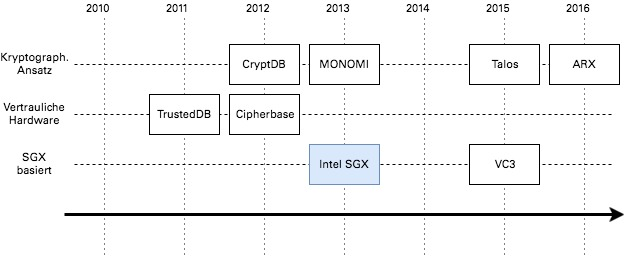
\includegraphics[width=0.9\linewidth]{img/RelatedWorkTimeline.pdf}
	\centering
	\caption{Zeitliche Einordnung verwandter Arbeiten nach Kategorie}
	\label{fig:timeline}
\end{figure}

TrustedDB \cite{Bajaj2013} erweitert den üblichen Datenbankserver um die zusätzliche Einbeziehung eines sicheren Koprozessors (SCPU), wie diese zum Beispiel von der Firma IBM hergestellt werden, um eine gesicherte Datenverarbeitung zu gewährleisten. Bei der Definition des Datenbankschemas können einzelne zu schützende Attribute entsprechend ausgezeichnet werden. Anhand von \ref{fig:trusteddb} wird die Funktionsweise des Verfahrens vereinfacht erklärt. 

\begin{figure}[h]
	\includegraphics[width=0.9\linewidth]{img/RelatedWorkTrustedDB.pdf}
	\centering
	\caption{Ablauf einer Datenbankanfrage unter TrustedDB}
	\label{fig:trusteddb}
\end{figure}

Bei einer Anfrage des Clients wird diese zunächst verschlüsselt, bevor sie zum Server gelangt (1). Der unsichere Teil des Servers kann die Anfrage in der Form nicht bearbeiten und leitet sie an die SCPU weiter. Nach der Entschlüsselung findet dort eine Unterteilung in Teilanfragen statt, unter dem Gesichtspunkt, ob diese die Verarbeitung sensibler oder harmloser Daten beinhalten (2). Resultat ist eine Menge sogenannter \textit{Public} und \textit{Private Queries}. Erstere kann die herkömmliche Datenbankengine übernehmen (3). Dies ist in der Regel ein deutlich größerer Anteil der Daten. Die SCPU übernimmt nur die private queries, also nur den Teil der Arbeit, für den sie tatsächlich bestimmt ist (4). Die Ergebnisse werden zum Schluss zusammengefügt und verschlüsselt zum Client zurückgeschickt (5), der diese wiederum entschlüsselt (6). Als großer Vorteil wird unter anderem die bessere Leistung gegenüber kryptographischer Berechnungen in Software beschrieben. Zudem gibt es keine Einschränkungen an möglichen \ac{SQL} Anfragen. Jedoch erfordert TrustedDBs Architektur das Einbetten eines gesamten Datenbanksystems in die SCPU und somit in die Trusted Computing Base. Aufgrund der beschränkten Ressourcen des Koprozessors muss hier zudem auf eine in Funktionalität ärmere SQLite Datenbank zurückgegriffen werden \cite{Arasu}. Sobald ein größerer Anteil der Daten als sensitiv eingestuft und die SCPU somit in größerem Maße beansprucht wird, nimmt die Leistung stark ab, da dessen Rechenleistung eingeschränkt ist \cite{Arasu2012}.

Im Gegensatz zu TrustedDB setzt Cipherbase \cite{Arasu2012}\cite{Arasu} auf einen sehr eng gekoppelten Ansatz und verspricht somit ein deutlich leistungsfähigeres System. Es erweitert ursprünglich den Microsoft \ac{SQL} Server um eine \textit{Trusted Machine}. Eine Besonderheit ist die Umsetzung jener als einfache Stapelmaschine, auf welcher ausschließlich die Berechnung der kryptographischen Primitive abläuft. Zur Realisierung der Trusted Machine eignen sich zum Beispiel \acp{FPGA} \cite{Arasu}. Kombiniert wird das ganze mit dem Einsatz einer eigenschaftserhaltenden Verschlüsselung, wie diese in später aufgeführten Verfahren wie CryptDB betrachtet wird. Man setzt hierbei auf ein statisches Modell, wodurch Data-at-rest einmalig mit der benötigten Methode unter Gewährleistung bestimmter Funktionalität, z.B. der Möglichkeit für Bereichsanfragen, verschlüsselt werden. Das enge Hardware Software Codesign erlaubt eine bessere Leistung gegenüber TrustedDB, während die \ac{TCB} möglichst klein gehalten wird \cite{Arasu}. Zudem gibt es keine Limitierungen in Bezug auf die unterstützte Ausdrucksmächtigkeit von Anfragen, da ein einziges umfangreiches Datenbanksystem erweitert wird \cite{Arasu2013}. Als Nachteil ist hier lediglich die Minderung gewisser Sicherheitsmerkmale im Zuge der eigenschaftserhaltenden Verschlüsselung zu nennen.

Auf Seiten der Verfahren, welche rein auf den eingesetzten Verschlüsselungsverfahren beruhen, ist an erster Stelle CryptDB \cite{Popa2011}\cite{Popa2012} zu nennen. Genau wie die zuvor behandelten Systeme erfolgte ein Entwurf für die Arbeit auf relationalen \ac{SQL} Datenbanken. Außerdem wurde es ebenso wie TrustedDB 2011 publiziert, wodurch die beiden Vorgehensweisen stets koexistierten. Der Kern von CryptDBs Architektur ist ein Proxy Server, der sich logisch gesehen zwischen Anwendungs- und Datenbankserver befindet, im Normalfall aber ebenfalls auf dem Anwendungsserver läuft. Sobald eine Anfrage an die verschlüsselte Datenbank gestellt wird oder eine Antwort zurückkommt, verlaufen diese zunächst über jenen Proxy. Ein vereinfachtes Schema der Architektur ist in Abbildung \ref{fig:cryptdb} zu sehen. CryptDB nutzt den Aufbau von \ac{SQL} Anfragen aus mehreren einfachen Operationen wie Joins, Gleichheitsprüfungen oder Ordnungen auf Werten aus, um diese direkt auf den verschlüsselten Daten durchführen zu können. Das entsprechend eingesetzte Schema wird als \textit{SQL aware encryption} bezeichnet. Es definiert kryptographische Methoden, unter dessen Einsatz der Erhalt einer bestimmten, auszuführenden Teilmenge von Operationen gewährleistet wird. Ist es beispielsweise nur nötig, eine Selektion mit Gleichheitsbedingung durchzuführen, so genügt ein deterministisches Verschlüsselungsverfahren, welches stets den gleichen Schlüsseltext für einen gegebenen Klartext produziert. Will man allerdings den minimalen oder maximalen Wert, bzw. eine geordnete Ergebnismenge erhalten, so muss ein schwächeres Verfahren eingesetzt werden, welches die Ordnung von Klartextwerten durch das Verschlüsseln erhält, sogenannte \ac{OPE}. Um eine möglichst große \ac{SQL} Funktionalität neben einem höchstmöglichen Maß an Vertraulichkeit bereitzustellen, setzt CryptDB auf ein sogenanntes \textit{Onion Scheme}. Data-at-rest ist in mehreren Schichten verschlüsselt, wobei die gegebene Sicherheit mit jeder Schicht zunimmt. Ebenso nehmen die möglichen Operationen ab. Entschlüsselt wird dann nur bis zu der Schicht, welche für die aktuellen Berechnungen erforderlich ist. Die benutzten Schlüssel liegen je Nutzer auf dem Anwendungsserver. Der Proxy selbst besitzt jedoch einen Masterkey, um Anfragen umschreiben zu können. Da jeder Benutzer des Systems über einen individuellen Schlüssel verfügt, ist es möglich, gewisse Daten für einzelne Nutzer freizugeben oder zu verstecken, wofür der Proxy ein spezielles Schema hält. Die Datenverarbeitung selbst erfolgt durch \acp{UDF} auf dem Datenbankserver, nachdem die eingehenden Anfragen umgeschrieben wurden. Infolge der Auslieferung von den verschlüsselten Ergebnisdaten an den Proxy, kann dieser die Entschlüsselung vornehmen und sie dem Anwendungsserver liefern.

\begin{figure}
	\includegraphics[width=0.9\linewidth]{img/RelatedWorkCryptDB.pdf}
	\centering
	\caption{Architektur von CryptDB}
	\label{fig:cryptdb}
\end{figure}

Trotz der zusätzlichen Bearbeitung im Proxy, hat CryptDB einen relativ geringen Overhead an Rechenaufwand im Vergleich zum herkömmlichen unsicheren Ablauf \cite{Popa2012}. Die Nachteile des Verfahrens liegen allerdings in den eingeschränkten Möglichkeiten an \ac{SQL} Anfragen, sowie den fehlenden Konfigurationsmöglichkeiten in Bezug auf die gewünschte Sicherheit. Eine absichtliche Nutzung schwächerer Verschlüsselungsverfahren wie \ac{OPE}, erleichtert einem Angreifer, Aussagen über die Schlüsseltexte zu treffen \cite{Poddar2016}. Als großer Nachteil ist auch zu nennen, dass im Gegensatz zu Cipherbase keine freie Konfiguration der Sicherheit je Spalte möglich ist.

Zwei Jahre nach der Veröffentlichung von CryptDB folgte mit MONOMI \cite{Tu2013} ein System, welches auf dem gleichen Verschlüsselungsschema aufbaute, jedoch für den Anwendungsfall von analytischen Workloads angepasst wurde. Diese unterscheiden sich größtenteils dadurch, dass viel größere Datenmengen auf komplexe Art verarbeitet werden. In einer komplett verschlüsselten Datenbank bringt dies viele Probleme mit sich, unter anderem, wie jene komplexen Anfragen effizient auf Schlüsseltexten ausgeführt werden können. Die Lösung von MONOMI besteht aus einer Verteilung der Anfrageausführung auf Server und Client. Bei Letzterem können somit letzte Verarbeitungsschritte ausgeführt werden, nachdem die Daten schon unverschlüsselt sind, während jene auf dem Server mit den verschlüsselten Daten deutlich aufwendiger wären. MONOMI bringt zudem noch weitere Leistungsoptimierungen mit und schneidet bei großen Benchmarks sowohl in Bezug auf Speicherbedarf und Leistung deutlich besser ab als CryptDB \cite{Tu2013}.

An dieser Stelle muss auch Talos \cite{Shafagh2015} erwähnt werden. Das 2015 beschriebene System vereinfacht und optimiert das Konzept von CryptDB für den Einsatz im Internet of Things. Die eingesetzten kryptographischen Algorithmen, z.B. für \ac{OPE} werden durch leistungsfähigere Varianten ersetzt und erlauben die Ausführung auf Systemen mit beschränktem Energiebudget und Speicherplatz.

Der letzte hier genannte Vertreter in der Reihe verwandter Arbeiten ist Arx \cite{Poddar2016}. Es handelt sich um einen ganz offiziellen Nachfolger von CryptDB, der 2016 veröffentlicht wurde. Diesmal verfolgte man eine neue Herangehensweise, indem man die Berechnungen nicht auf eigenschaftserhaltenden Verschlüsselungsverfahren, sondern auf speziellen Datenstrukturen aufsetzt. Dies erlaubt es, komplett unabhängig von einer Art der Verschlüsselung zu sein und ausschließlich starke, bzw. anerkannte Standardverfahren wie den \ac{AES} zu nutzen. Arx nutzt spezielle Datenbankindizes, welche speziell zum Traversieren verschlüsselter Daten entworfen wurden und die Sicherheit dahingehend gewähren, dass die Knoten in den Indexstrukturen nach jeder Benutzung zerstört und entsprechend erneuert werden müssen.

In diesem Abschnitt wurden die zwei generellen Ansätze zur Umsetzung eines sicheren Datenbanksystems, und die wichtigsten Vertreter auf beiden Seiten betrachtet. Der Einsatz von dedizierter Hardware als sicherer Vertrauensbereich zur Datenverarbeitung erlaubt eine große Flexibilität in Bezug auf Konfigurierbarkeit und verfügbare Operationen. Demgegenüber steht die mit oftmals hohen Kosten verbundene Integration jener Komponenten in das Gesamtsystem, sowie die begrenzten sicheren Speicher- und Rechenkapazitäten als Flaschenhals. Die Nutzung von eigenschaftserhaltenden Verschlüsselungsschemata und speziellen Datenstrukturen hingegen erlaubt eine schnellere Lösung in Software, allerdings auf Kosten des Sicherheitsgrades und der Funktionalität. Die Kombination beider Ansätze, etwa in Cipherbase, sorgt dafür, dass nur ein möglichst kleiner Teil an Berechnungen in der sicheren Hardware ausgeführt wird und bietet somit einen Kompromiss der jeweiligen Vor- und Nachteile.

\section{Intel SGX im Kontext sicherer Datenbanken}

Nachdem ein Überblick über bestehende Ansätze zur Lösung des Problems eines sicheren Umgangs mit Daten in einer Datenbank erklärt wurden, wird nun die in dieser Arbeit zentrale Technologie vorgestellt. Wie auch schon bei den Vertretern TrustedDB und Cipherbase, steht der Einsatz einer vertrauenswürdigen Hardwarekomponente im Mittelpunkt, mit der Absicht, eine sichere Datenspeicherung und -verarbeitung in einem potenziell böswilligen Umfeld durchführen zu können. Während die zuvor genannten Ansätze jedoch die Integration zusätzlicher Hardware voraussetzten, geschieht dies in diesem Fall komplett auf einem gebräuchlichen Intel Prozessor.
Erstmals 2013 von Intel beschrieben \cite{McKeen2013}, sind die als \ac{SGX} veröffentlichten x86 Architekturerweiterungen im Herbst 2015 als Teil der 6. Generation Intel Core Prozessoren (Codename Skylake) erschienen \cite{Aumasson2016}. In diesem Abschnitt soll ein Überblick über das Konzept und die allgemeine Funktionsweise von Intel \ac{SGX} gegeben werden. Zunächst wird dabei auf die technischen Grundbestandteile eingegangen. Ein besonderes Merkmal von \ac{SGX} ist die Möglichkeit der \textit{remote attestation}, welche es einem Client ermöglicht, sicherzustellen, dass er auch wirklich mit dem beabsichtigtem Teil der Software in einem sicheren Bereich auf dem entfernten Server interagiert.

Die Grundlage der Funktionalität von \ac{SGX} ist die Definition einer eigenen, kontinuierlichen Region im physischen Hauptspeicher des entsprechenden Systems. Diese wird als \ac{PRM} bezeichnet und beherbergt die sogenannten Enclaves, sichere Einheiten zur Verwahrung von sensiblem Code und Daten. Jede Enclave kann dabei als ein abgeschlossener, verschlüsselter Container betrachtet werden. Die \ac{CPU} schützt den \ac{PRM} vor sämtlichen Zugriffen, welche nicht von einer Enclave ausgehen, sei es von Seiten des Kernels, Hypervisors, durch Peripheriegeräte oder sonstiger (privilegierter) Systemkomponenten. Die Speicherseiten der einzelnen Enclaves sind im \ac{EPC} verwahrt, welcher im PRM beinhaltet ist. Metadaten zu jeder \ac{EPC} Seite werden in einem \ac{EPCM}, einer Datenstruktur im Prozessor selbst, mitgeführt. Ein Schema, welches die eben eingeführten Komponenten zusammenhängend darstellt, ist in Abbildung \ref{fig:intelsgxmemory1} zu sehen.

\begin{figure}
	\includegraphics[width=0.9\linewidth]{img/IntelSGXMemory1.pdf}
	\centering
	\caption{Zusammenhang von PRM, EPC und EPCM}
	\label{fig:intelsgxmemory1}
\end{figure}

Die Anwendungssoftware kann eine oder mehrere Enclaves einbinden, um sie zur sicheren Datenspeicherung und Berechnung zu nutzen. Dieser Vorgang beginnt zunächst mit einer Einrichtung der jeweiligen Enclave. Deren initialer Inhalt wird zunächst von der \ac{CPU} in den \ac{PRM} transferiert, woraufhin die nicht vertrauenswürdige Systemsoftware jene \ac{EPC} Seiten alloziert und der zu ladenden Enclave zuordnet. Um zu verhindern, dass die Sicherheitsgarantien trotz Einbeziehung des Betriebssystems eingehalten werden können, wird im \ac{EPCM} vermerkt, welcher Enclave jede EPC Seite angehört. Der Prozessor kann somit prüfen, ob die Allokation korrekt durchgeführt wurde, oder etwa eine Seite mehrfach zugeteilt wurde. Die jeweils erste allozierte Seite dient einer Unterbringung der \ac{SECS}, welche Metadaten der entsprechenden Enclave beinhaltet und ab diesem Zeitpunkt zu deren Referenzierung dient. Nach Vollendung der Prozedur wird die Enclave als initialisiert gekennzeichnet und der sogenannte \textit{Measurement Hash} vollendet, ein kryptographischer Hash des Enclaveinhalts, welcher zu Zwecken der Attestierung benötigt wird. Außerdem am Startprozess beteiligt ist stets die sogenannte \textit{Launch Enclave}, welche durch Intel für das Laden anderer Enclaves bereitgestellt wird, und als Teil eines Systemdienstes im Hintergrund läuft. Ihr zusätzlicher Zweck ist es, den Start einer Enclave zu autorisieren. Im produktiven Umfeld eingesetzte Enclaves müssen sich nämlich einer offiziellen Lizenzierung durch Intel unterziehen \cite{Costan2016}.

Nach dem Laden der Enclave, befindet sie sich im \ac{PRM} und Adressraum des jeweiligen Nutzerprozesses. Innerhalb der einsatzbereiten Enclave befinden sich nun ihr eigener privater Code und private Daten. Das vorliegende Adressraumschema ist vereinfacht in Abbildung \ref{fig:intelsgxmemory2} gezeigt. Jegliche Berechnungen, sowie gespeicherte Daten innerhalb der Grenzen einer einzelnen Enclave sind durch die \ac{CPU} geschützt. Sämtlicher Inhalt ist zudem durch eine oder mehrere dedizierte Hardwarekomponenten, den \textit{Memory Encryption Engines} verschlüsselt und kann nur innerhalb der \ac{CPU} entschlüsselt werden, was es unmöglich macht, Informationen durch das Auslesen des Speichers zu gewinnen \cite{McKeen2013}. Sobald ihre Funktionalität beansprucht wird, sprich der Ausführungsfluss die Enclave passieren will, sind spezielle \ac{CPU} Instruktionen notwendig. Der hierfür eingesetzte Mechanismus ist ähnlich dem Sprung vom User- in den Kernel Mode. \ac{SGX} unterstützt zudem Multithreading, wodurch sich mehrere Threads parallel in einer Enclave befinden können. Je zu unterstützendem logischen Prozessor erfordert dies das Anlegen von Metadaten in einer \ac{TCS}, welche jeweils eine \ac{EPC} Seite füllt. Der Zweck liegt darin, dass der Ausführungspfad eines Threads innerhalb der Enclave genauestens bekannt und somit dokumentiert sein muss, um ihn in den Measurement Hash eingehen zu lassen \cite{McKeen2013}.

\begin{figure}
	\includegraphics[width=0.6\linewidth]{img/IntelSGXMemory2.pdf}
	\centering
	\caption{Adressraumschema nach Einbindung sicherer Enclaves}
	\label{fig:intelsgxmemory2}
\end{figure}

Da die Enclave selbst aus dem unsicheren Speicher geladen wird, ist ihr initialer Zustand nach außen hin bekannt. Die sichere Verwendung findet folglich erst nach der Initialisierung statt. Es ist jedoch im Interesse eines Nutzers, zu wissen, ob das Stück Software auf dem entfernten System, welches seine Daten bearbeiten soll, auch seinen Erwartungen entspricht. \ac{SGX} erlaubt es, mithilfe der remote attestation eine Integritätsprüfung auf dem Inhalt der Enclave durchführen zu lassen. Hierbei kommt ein asymmetrisches Verschlüsselungsverfahren zum Signieren ihres Measurements zum Einsatz \cite{Costan2016}. Der Nutzer kann diese Signatur prüfen und somit die Integrität der Gegenseite bewerten. Die für den ganzen Vorgang benötigten \textit{Attestation Keys} werden von Intel selbst ausgestellt \cite{Johnson2016}.

Der sicherlich größte Unterschied zu allen zuvor betrachteten Entwicklungen, welche auf Vertrauensbereiche in Hardware setzen, ist die Einbeziehung bereits in jedem System vorhandener Hardwarekomponenten, genauer gesagt des Hauptspeichers und vor allem des Prozessors. Letzterer bildet somit, zusätzlich zu sämtlichen zur Attestierung notwendigen Softwarebestandteilen die allgemeine \ac{TCB}. Es muss somit auf die korrekte Funktionsweise des Intel Prozessors vertraut werden, was allerdings zwangsläufig der Fall ist, da er für die Ausführung von Programmen zuständig ist und seine interne Logik ohnehin schwer überprüft werden kann \cite{Aumasson2016}. Unter Nutzung von \ac{SGX} können bereits vorhandene Systeme ohne eine große Aufrüstung durch zusätzliche Hardware um eine Komponente zur sicheren Datenverarbeitung erweitert werden. Interessant ist hierbei natürlich, welche Eigenschaften die Enclaves in Bezug auf zur Verfügung stehendem Speicher, Leistungsaufwand bei Berechnungen, oder Möglichkeiten bei der Programmierung aufzeigen. Entsprechende Untersuchungen werden als Hauptaugenmerk dieser Arbeit in späteren Kapiteln betrachtet.

\section{Fazit}

In diesem Kapitel wurde die Datensicherheit aus Sicht eines Datenbanksystems behandelt. Um die drei Schutzziele Vertraulichkeit, Integrität und Verfügbarkeit zu gewährleisten, wurde klassischerweise auf ein hierarchisch organisiertes Prinzip gesetzt. Der physische Schutz des Systems bildet die Grundlage der Sicherheit des Betriebssystems, welche wiederum erforderlich ist, um das Datenbanksystem zu schützen. Jede Schicht verfügt über eigene Maßnahmen, um dieses Ziel zu erreichen. Im Kontext von cloudbasierten Datenbanken ist jenes konventionelle Prinzip jedoch nicht mehr ausreichend, da sowohl die physische Hardware als auch das Betriebssystem unter der Kontrolle eines Dritten stehen. Um dennoch die Vertraulichkeit und Integrität von Data-at-rest und Data-in-use garantieren zu können, ergeben sich gewisse Anforderungen an das Datenbanksystem. Ruhende Daten müssen in verschlüsselter Form vorliegen und die Datenverarbeitung muss auf eine Weise stattfinden, dass keine Klartextdaten von einem Angreifer ausgelesen werden können. In der Vergangenheit haben sich zwei allgemeine Ansätze gebildet, um ein derartiges System zu entwerfen. In Vertretern wie TrustedDB und Cipherbase setzt man vorrangig auf die Einbeziehung von zusätzlicher Hardware, um Bereiche zu schaffen, in denen gesicherte Berechnungen auf Klartexten stattfinden können. Publikationen zu CryptDB oder Arx hingegen nutzen lediglich spezielle Verschlüsselungsschemata und Datenstrukturen, um verarbeitende Operationen direkt auf Schlüsseltexten durchzuführen. Intel \ac{SGX} ist eine aktuelle Lösung des Prozessorherstellers, welche den Ansatz der Vertrauensbereiche in einen handelsüblichen Prozessor integriert. Dieser nutzt einen gesicherten Bereich im Hauptspeicher und schützt ihn vor sämtlichen Zugriffen von außen, inklusive jener von privilegierten Komponenten wie dem Kernel oder Hypervisor.
% 3. Kompression

\chapter{Kompression}

Kompression ist ein weitverbreitetes Mittel zur Erzielung von Leistungsverbesserungen im Bereich der Datenverarbeitung. Einen zunehmenden Einsatz fanden sie vor allem in den immer stärker verbreiteten In-Memory Datenbanken, welche sämtliche Daten nicht wie zuvor üblich auf der Festplatte speichern, sondern den deutlich schneller verfügbaren Hauptspeicher nutzen.

Wie bereits im letzten Kapitel beschrieben, hat Intel mit seinen Secure Guard Extensions die Möglichkeit geschaffen, Daten innerhalb von sicheren Vertrauensbereiche (Enclaves) zu verarbeiten. Dies ermöglicht es mitunter, eine Umgebung zu schaffen, in welcher auf verschlüsselten Informationen ohne Beeinträchtigung der Vertraulichkeit im Klartext gerechnet werden kann. Der zusätzliche Einsatz von Kompressionsverfahren kann in diesem Szenario sinnvoll sein, um die Transferzeiten von Daten in eine Enclave, sowie den zeitlichen Verlust durch kryptographischen Operationen, je durch eine höhere Datendichte, zu verringern.

Im aktuellen Kapitel soll ein Einblick in den Einsatz und die Funktionsweise von Kompressionsverfahren in Datenbanksystemen gegeben werden. Zunächst wird etwas genauer auf die grundlegende Motivation ihres Einsatzes in diesem Kontext eingegangen. Verwandte Arbeiten zu dem Thema und eine damit verbundene zeitliche Darstellung der Forschungsentwicklungen wird nachfolgend beleuchtet, gefolgt von der Betrachtung konkreter Algorithmen. Letztere sind von besonderer Relevanz, da sie den Kern der Untersuchungen dieser Arbeit darstellen und später in einer SGX Enclave zum Einsatz kommen werden.

\section{Grundlagen}

Durch das Verdichten von Daten, erlauben Kompressionsverfahren eine effizientere Nutzung der Ressource Speicher zugunsten der Datenverarbeitungszeit. Somit begünstigen sie eine bessere Ausnutzung der Speicherhierarchie, an deren Spitze die kleinen Prozessorregister mit schnellen Zugriffszeiten stehen und die Basis durch große, aber vergleichsweise sehr langsame Festplattenspeicher gebildet wird. Von Vorteil ist hierbei die Möglichkeit, eine höhere weil dichtere Datenmenge auf dem gleichen physischen Speicherplatz, etwa dem Prozessorcache, zu halten. Zudem werden Datentransferraten zwischen den einzelnen Stufen der Hierarchie erhöht \cite{Croft2009}. Zugrundeliegend ist ein \textit{Time-Memory Tradeoff}, denn die Einsparung an Speicherplatz kommt auf Kosten zusätzlicher Berechnungszeit dadurch, dass die Daten vor der eigentlichen Verarbeitung dekomprimiert werden müssen.

Durch ihre Arbeit auf dem Hauptspeicher nutzen In-Memory Datenbanken bereits eine höhere Stufe der Speicherhierarchie, als dies bei festplattenbasierten System der Fall ist. Um die Verarbeitungsgeschwindigkeit weiter zu verbessern, ist es nötig, die Transferzeiten von Daten zur \ac{CPU} weitestgehend zu verringern. Eine größtmögliche Komprimierungsrate durch den Einsatz von Verfahren wie Huffman oder Lempel-Ziv anzustreben, erscheint aber keineswegs sinnvoll, da die zeitlichen Einsparungen in Bezug auf die zu transferierende Datenmenge durch den Zwang der aufwendigen Dekomprimierung zunichte gemacht werden \cite{Abadi2006}. Notwendig sind demnach leichtgewichtige Verfahren, sodass sich Daten schnell genug dekomprimieren lassen, um insgesamt echte Leistungsverbesserungen zu erzielen. Einige Verfahren wie die Lauflängenkodierung erlauben sogar die schnellere Verarbeitung auf komprimierten Daten selbst.

\section{Verwandte Arbeiten}

Die ersten Untersuchungen über den Einsatz von Kompressionstechniken in großen Datenbanken wurden 1982 veröffentlicht. Eine Gesamtverringerung der Datenmenge von 30-90\% war ein vielversprechendes Ergebnis, obwohl jene Verfahren zu jener Zeit noch kaum genutzt wurden \cite{Severance1982}. Des weiteren wurde gezeigt, dass gespeicherte Daten verschiedene Eigenschaften besitzen, welche manche Kompressionsverfahren eher begünstigen als andere.

In späteren Publikationen bedachte man nun nicht nur mehr die reine Datenhaltung, sondern auch die Nutzung zur effizienteren Datenverarbeitung im \textit{Query Processing}. Da eine Dekomprimierung vor Berechnungen obligatorisch ist, geht der Vorteil von Einsparung an Speicherplatz in gewissen Maßen verloren. Beschrieben wurden daher Kompressionsverfahren, welche es erlaubten, soweit wie möglich direkt auf den komprimieren Daten zu arbeiten um den verfügbaren Speicher möglichst effektiv zu nutzen \cite{Graefe1991}.

Allgemein adressierten frühere Ansätze vor allem traditionell relationale Datenbanksysteme, wobei die zu komprimierenden Einheiten etwa einzelne Tabellenreihen darstellten. Die in den letzten Jahren stark aufstrebenden spaltenorientierten Datenbanken bieten hingegen ein höheres Potenzial zur Kompression, dadurch, dass benachbart gespeicherte Werte in der Regel einer Spalte angehören und den gleichen Datentyp besitzen \cite{Abadi2006}. Besonders geeignet sind in diesem Fall Kompressionsschemata, welche auf Datenlokalität, also das enge Beieinanderliegen ähnlicher Daten, beruhen. Es wurde zudem gezeigt, dass das physische Datenbankdesign und das eingesetzte Verfahren zur Kompression auf einander abgestimmt sein müssen, um die besten Leistungsverbesserungen zu erzielen. Entsprechend spielt die Natur des zu erwartenden \textit{Query Workloads} eine entscheidende Rolle bei dessen Auswahl für jede individuelle Spalte.

\section{Algorithmen}

Die Grundlage von verlustfreier Kompression stellt die Darstellung einer Eingabesequenz an Daten in einer verkürzten Form dar, indem gewisse überschüssige Informationen, wie sie etwa durch Redundanz entstehen, reduziert werden. Es lassen sich verschiedene Herangehensweisen unterteilen, welche einzeln oder in kombinierter Form bei Kompressionsverfahren zum Einsatz kommen \cite{Abadi2006}\cite{Croft2009}:

\subparagraph{Nullunterdrückung}
Führende Leerstellen bzw. Nullen in der binären Repräsentation werden entfernt und durch entsprechende Angaben zu deren Anzahl und der Position des Auftretens ersetzt.

\subparagraph{Deltakodierung}
Gespeichert werden lediglich die Differenzen aufeinanderfolgender Werte, da diese in manchen Szenarien deutlich kleiner ausfallen, als die (absoluten) Werte selbst.

\subparagraph{Wörterbuchkodierung}
Es erfolgt eine eindeutige Abbildung häufig auftretender Sequenzen auf kürzere Codes.

\subparagraph{Lauflängenkodierung}
Abfolgen gleicher Werte werden durch eine einzige Darstellung bestehend aus Wert und Lauflänge ersetzt.

\subparagraph{Bitvektorkodierung}
Anstatt der Folge von Werten selbst, werden jeweils die Positionen des Auftretens jedes Wertes kodiert, sodass jeder Wert einen individuellen Bitvektor besitzt.

\paragraph{}
In diesem Unterkapitel soll mit VByte ein konkreter einfacher Algorithmus behandelt werden, welcher sich die Nullunterdrückung zunutze macht. Anschließend wird ein möglicher Ansatz zur Lauflängenkodierung untersucht und auf seine besonderen Eigenschaften bei der Datenverarbeitung eingegangen.

\subsection{VByte}

Bei VByte \cite{Croft2009} (abgeleitet von \textit{variable byte length}) handelt es sich um ein äußerst schnelles Verfahren, welches kleinere Zahlenwerte kürzer kodiert als längere. Der Einsatz eignet sich demzufolge immer dann, wenn die vorliegende Eingangssequenz aus vielen kleineren Integern besteht. Der Algorithmus arbeitet byteorientiert, wodurch die Ausgabe stets ein Vielfaches eines Bytes ist und der kleinstmögliche Code genau ein Byte lang ist. Als Eingabe dienen 32 Bit Integerwerte, welche auf bis zu 5 Byte abgebildet werden.

Das generelle Vorgehen bei der Komprimierung besteht aus dem Prüfen der numerischen Größe des 32 Bit Wertes. Hierdurch kann eine Aussage über die Anzahl führender Nullen getroffen werden, welche es zu entfernen gilt. Um zu Zwecken der späteren Dekomprimierung zu kennzeichnen, welche Bytes durch die Nullunterdrückung entfallen sind, wird jedes Ausgabebyte durch 7 Datenbits und einen Deskriptor im obersten Bit kodiert. Letzteres dient der Anzeige des aktuellen Laufs: eine 1 bedeutet, dass das Byte noch Teil des aktuellen Wertes ist, während eine 0 den Anfang eines neuen Integers indiziert. Entsprechend werden jegliche Werte kleiner gleich $2^7$ durch ein Byte kodiert, jene kleiner gleich $2^{14}$ durch zwei Byte und so weiter. In Abbildung \ref{fig:vbyte} wird die beispielhafte Komprimierung des Integers 0x000D9E5B (32 Bit) in der hexadezimalen Repräsentation gezeigt. Durch Einsparung des ersten Bytes und Berücksichtigung der zusätzlichen Deskriptorbits (grau gekennzeichnet) resultiert die Ausgabe 0x36BCDB (24 Bit).

\begin{figure}
	\includegraphics[width=\linewidth]{img/VByte.pdf}
	\centering
	\caption{Beispiel zur VByte Kompression}
	\label{fig:vbyte}
\end{figure}

\subsection{Lauflängenkodierung}

Anders als VByte sind Verfahren der Lauflängenkodierung \cite{Reghbati1981} (oder \ac{RLE}) nicht zwangsläufig byteorientiert. Der Einsatz des Verfahrens ist immer dann sinnvoll, wenn Werte oftmals wiederholt nacheinander auftreten, etwa in einer der Größe nach sortierten Folge von Integern. Entsprechende Redundanz kann genutzt werden, um jene Sequenzen in Läufe zu unterteilen. Anstatt die aufeinanderfolgenden wiederholten Werte speichert man nur noch Tupel der Form (Wert, Lauflänge). In Abbildung \ref{fig:rle} wird eine beispielhafte Komprimierung der Folge 11123344555 durchgeführt. Man kann leicht erkennen, dass das einfache Auftreten eines Wertes in einem jeweils längeren Code resultiert und eine echte Verkürzung erst ab der Lauflänge 3 erfolgt. Anders als in dem abgebildetem Schema, müssen die Lauflängenwerte jedoch nicht die gleiche Größe wie die Ausgangswerte haben. Je nachdem wie wahrscheinlich die maximal zu erwartende Lauflänge ist, können sie deutlich kleiner gewählt werden, um die Kompressionsrate weiter zu erhöhen. Es existieren auch weitere Optimierungsmöglichkeiten wie beispielsweise das Einsparen der Komprimierung bei kleineren Lauflängen.

\begin{figure}
	\includegraphics[width=0.9\linewidth]{img/RLE.pdf}
	\centering
	\caption{Beispiel zur RLE Kompression}
	\label{fig:rle}
\end{figure}

Sofern eine Integerwertefolge durch die Komprimierung mittels \ac{RLE} verdichtet wurde, wird in gleichem Maße die Bildung des Summenaggregats begünstigt. Anstatt die Werte einzeln aufzusummieren, bietet sich hierbei ein direktes Arbeiten auf den komprimierten Werten an, da Additionen durch die Berechnung von $Wert * Laufl\ddot{a}nge$ eingespart werden können. Im Beispiel von Abbildung \ref{fig:rle} ergeben sich 10 Operationen durch die Berechnung auf den unkomprimierten Werten:

\begin{equation*}
	1 + 1 + 1 + 2 + 3 + 3 + 4 + 4 + 5 + 5 + 5 = 34
\end{equation*}

Für entsprechende Berechnung auf komprimierten Werten sind nur 9 Operationen notwendig, während Berechnungskosten für die Dekomprimierung entfallen:

\begin{equation*}
	1 * 3 + 2 * 1 + 3 * 2 + 4 * 2 + 5 * 3 = 34
\end{equation*}

\section{Fazit}
%TODO


\paragraph{}
%In diesem und dem vorhergehenden Kapitel wurden mit der Sicherheit in Datenbanksystemen und der Kompression als Hilfsmittel in der Datenverarbeitung die grundlegenden Konzepte dieser Arbeit untersucht. Neben verschiedenen Ansätzen zur Gewährleistung der Vertraulichkeit wurde Intel \ac{SGX} als aktuelle auf Hardware basierende Entwicklung eingeführt, welche sich die Definition von Enclaves als sichere, nur durch den Prozessor zugreifbare Vertrauensbereiche zunutze macht. Die Platzbeschränkungen sowie Transferzeiten von Daten in jene Bereiche gestalten sich als Herausforderungen, welchen durch eine Datenkompression entgegengewirkt werden kann. Daher wurde eine entsprechende Einführung in den bestehenden Einsatz von Kompressionsverfahren innerhalb datenverarbeitender Systeme gegeben und einige Herangehensweisen zu deren Umsetzung erklärt. Zur Nutzung in den folgenden Untersuchungen dieser Arbeit waren abschließend zwei konkrete Algorithmen, VByte und ein Lauflängenkodierungsverfahren, im Fokus.
%TODO Outro ggf. überarbeiten, um die Arbeit richtig abzurunden
% 4. Implementierung

\chapter{Implementierung}
%TODO intro

\section{Benutzung von Intel SGX}
%TODO notes

\section{Systemtest}
%TODO notes

\section{Fazit}
%TODO notes
% 5. Evaluierung

\chapter{Evaluierung}
%TODO intro

\section{Konzept}
%TODO notes

% \section{Punkt 1}
% \section{Punkt 2}
% \section{Punkt 3} ...

\section{Fazit}
%TODO notes
% 6. Fazit

\chapter{Fazit und Ausblick}
%TODO notes

\newpage
\bibliographystyle{plaindin}
\bibliography{library} 

\end{document}